\clearpage{}
\section{Discuss the principles of code reviews. Describe the principles of
formal program proofs. Define test cases, test suites, test equivalence
classes. Discuss functional and structural test objectives. Define the
notion of code coverage and explain some coverage criteria.}


\subsection{Principles of code reviews}

Similar to requirements and design reviews. \newline
Review code and documentation. \newline

Team: the programmer(s) + 3--4 experts (no customer because they are not concerned with the implementation).

\paragraph{Code walkthrough: less formal}
The programmer presents the code and documentation and the team comments on
correctness.

\paragraph{Code inspection: more formal}

List of review concerns (data types, algorithms, comments, etc\ldots)
Overview meeting -> individual review -> report meeting
Lead by a moderator (not the programmer) \newline

Experience show that code review is very effective at detecting faults.

\subsection{Principles of formal program proofs}

Prove code correctness, by proving that program respect the specifications formally.
\begin{itemize}
	\item Specifications: pre/post conditions as formal, logical statements
	\item Programs as flow graph of formal steps
\end{itemize}
\subsubsection{Inductive assertions method}
\todo{Add graph}
\begin{enumerate}
	\item Start from program flow chart
	\item Annotate endpoint node with pre-condition and post condition
	\item Annotate each loop with loop invariant
	\item For every basic path p from $A_i$ to $A_j$:
	\begin{itemize}
		\item compute the weakest precondition $wp(p,A_j)$ by propagating $A_j$
		back through all the steps of p prove that $A_i \rightarrow wp(p,A_j)$
	\end{itemize}
\end{enumerate}

\subsubsection{Symbolic Execution}
\begin{itemize}
	\item Variables receive symbolic values
	\item Execution state = symbolic values + conditions (start = inially symbol + pre\_cond
	\item Execute program paths symbolically (update variable and conditions)
	\item Check that final state satisfies post-conditions
\end{itemize}

\subsubsection{Advantages and Desadvantages}
\begin{itemize}
    \item[+] Gives a formal understanding of the program
    \item[+] Strong guarantee of correctness
    \item[-] Much work (more than writing the program) writing assertions, carrying the proofs
    \item[-] More complex programs are harder to prove data structures, pointers, concurrency,\ldots
    \item[-] Only proves assertions
    \item[-] Proofs can be faulty
\end{itemize}

\subsection{Test definitions}

\begin{description}
    \item[Test case (or test point)] Test an output for an input
    \item[Test suite] A series of test cases.
    \item[Test equivalence classes] The space of possible inputs $X$ is partitioned into equivalence classes $x \approx x'$ iff $x$ and $x'$ will detect the same faults.
    \item[Goal] choose one test case in each equivalence class (more than one => redundant; less than one => incomplete).
\end{description}

\subsection{Functional and structural test objectives}
The test objectives can be functional or structural. \newline

\begin{description}
    \item[Functional] Test cases based on functional specifications.
        \subitem{} All functions are performed correctly => black box.
    \item[Structural] Test cases based on code structure (test the branches).
        \subitem{} All statements are executed correctly => white-box.
\end{description}


\subsection{Code coverage}

\paragraph{Coverage criteria:}
In relation with structural test, to measure what parts of the code have been
exercised/tested.

\begin{itemize}
    \item Statement coverage: all program statements
    \item Branch coverage: all program branches
    \item Path coverage: all program paths
\end{itemize}
Some coverage cases may be unfeasible:
\begin{itemize}
	\item if (x = 1) \{ .../*A*/\}
	\item if (x \% 2 == 0) \{.../*B*/\}
\end{itemize}

$\rightarrow$ impossible in general (unbounded loop)

\paragraph{Def-use coverage criteria:}

\begin{itemize}
    \item Def-use pair: from a variable definition to a use of that variable that is reachable from this definition.
    \item All-uses coverage: all def-use pairs
    \item Def-use path coverage: all paths of all def-use pairs.
\end{itemize}

Also distinguish predicate and computational uses\ldots

\begin{figure}[!ht]
    \centering
    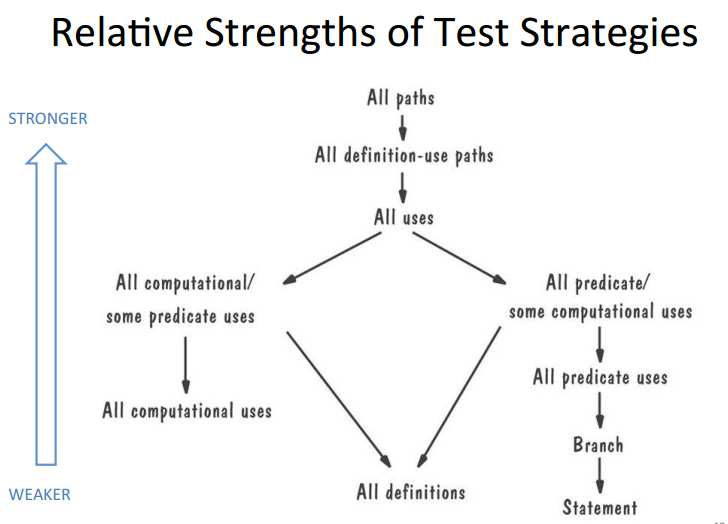
\includegraphics[width=0.6\linewidth]{strength_test_strategies.png}
\end{figure}
